% vim:ts=4:sw=4
%
% Copyright (c) 2008-2009 solvethis
% Copyright (c) 2010-2015 Casper Ti. Vector
% Public domain.
%
% 使用前请先仔细阅读 impthss 和 biblatex-caspervector 的文档,
% 特别是其中的 FAQ 部分和用红色强调的部分。
% 两者可在终端/命令提示符中用
%   texdoc impthss
%   texdoc biblatex-caspervector
% 调出。

% 采用了自定义的(包括大小写不同于原文件的)字体文件名,
% 并改动 ctex.cfg 等配置文件的用户请自行加入 nofonts 选项;
% 其它用户不用加入 nofonts 选项,加入之后反而会产生错误。
%
% 图书馆要求电子版论文的目录必须为黑色,
% 且某些教务要求打印版论文的文字部分为纯黑色而非灰度打印,
% 【因此最终打印和提交论文前,请将“colorlinks”改为“nocolorlinks”。】
\documentclass[UTF8, nocolorlinks, openany, spacing, pdftoc, pkuspace]{impthss}
% 设置行距为1.5。ctex说明文档中说linespread也可以作为选项传入,但测试结果显示不起效果。
% 因此在此处显示调用\linespread命令设置行距,测试显示有效果。
\linespread{1.5}
% 使用 biblatex 排版参考文献,并规定其格式(详见 biblatex-caspervector 的文档)。
% 这里按照英文文献在前,中文文献在后排序(“sorting = ecnty”);
% 若需按照中文文献在前,英文文献在后排序,请设置“sorting = centy”;
% 若需按照引用顺序排序,请设置“sorting = none”。
\usepackage[backend = biber, style = caspervector, utf8, sorting = none]{biblatex}
% 提供近似于学校所要求的 Times New Roman / Arial 的字体。
\usepackage[defaultsups]{newtxtext}
\usepackage{newtxmath}
% 产生 originauth.tex 里的 \square。
\usepackage{latexsym}

% 按学校要求设定参考文献列表中的条目之内及之间的距离。
\setlength{\bibitemsep}{3bp}
% 对于 linespread 值的计算过程有兴趣的同学可以参考 impthss-extra.sty。
\renewcommand*{\bibfont}{\zihao{5}\linespread{1.27}\selectfont}

% 设定文档的基本信息。
% \ctexset{today=big}
\impthssinfo{
	cthesisname = {博士研究生学位论文}, ethesisname = {Doctor Thesis},
	ctitle = {用于空间暗物质探测的塑闪阵列探测器的设计与研制},
	etitle = {Doctor Thesis \LaTeX{} Template for the Institute of Modern Physics of Chineses Academy of Sciences},
	cauthor = {周勇},
	eauthor = {Zhou Yong},
	studentid = {0123456789},
	date = {\today},
	school = {中国科学院大学研究生院},
	cmajor = {粒子物理与原子核物理}, emajor = {Nuclear and Particle Physics},
	direction = {实验核物理},
	cmentor = {孙志宇教授}, ementor = {Prof.\ Sun Zhiyu},
	ckeywords = {其一,其二}, ekeywords = {KeywdOne, KeywdTwo}
}
% 载入参考文献数据库(注意不要省略“.bib”)。
%\addbibresource{thesis.bib}
\addbibresource{./refs/ch2.bib}
\addbibresource{./refs/ch3.bib}
\addbibresource{./refs/ch4.bib}

% extra packages
\usepackage[absolute, overlay]{textpos} %封面制作
% \usepackage{import} % 使用\import,\subimport命令模块化文档结构,可以用相对路径载入文档
\usepackage{blindtext}
\usepackage{comment}
\usepackage{siunitx}
\usepackage{float}
\usepackage{mdwlist}
% \usepackage{subcaption} //error
% 表格内角注
\usepackage{threeparttable}
\AtBeginEnvironment{tablenotes}{\small}{}{}
% 设置表格字体大小
\usepackage[font=normalsize]{caption}
\let\oldtabular\tabular 
\renewcommand{\tabular}{\small\oldtabular}

\raggedbottom
\begin{comment}
	\usepackage{etoolbox}
	\newskip\mfilskip
	\mfilskip=0pt plus 3cm\relax
	\newcommand{\mfilbreak}{\vspace{\mfilskip}\penalty -200%
	\ifdim\lastskip<\mfilskip\vspace{-\lastskip}\else\vspace{-\mfilskip}\fi}
	\pretocmd{\section}{\mfilbreak}{}{}content...
\end{comment}

% 处理tiff图片
% \usepackage{grfext}
% \DeclareGraphicsRule{.tif}{png}{.png}%
% {%
  % `convert #1 `dirname #1`/`basename #1 .tif`-tif-converted-to.png %
% }

% \includeonly{./chap/introduction/introduction}
% \includeonly{./chap/description/description}
% \includeonly{./chap/dynamic_range/dynamic_range}
\includeonly{./chap/introduction/introduction,./chap/description/description,./chap/dynamic_range/dynamic_range,./chap/pmt_test/pmt_test,./chap/construction/construction,./chap/appendix/app1}
\begin{document}
	%%%%%%%%%%%%%%%%%%%%%%%%%
	%%% 封面,版权,声明,致谢 %%%
	\covermatter
	% 自动生成封面。
%	\maketitle
	% 从pdf载入封面
 	\begin{textblock*}{210mm}(0mm, 0mm)
\begin{figure*}[!hbt]
	\centering
	% 
\includegraphics[width=210mm]{fig/ucas_cover_cn.eps}
	
\includegraphics[width=210mm]{fig/lzu_cover.eps}
\end{figure*}
\end{textblock*}

 	\null\newpage
 	\begin{textblock*}{210mm}(0mm, 0mm)
\begin{figure*}[!hbt]
	\centering
	
\includegraphics[width=210mm]{fig/ucas_cover_en.eps}
\end{figure*}
\end{textblock*}


 	\null\newpage

	% 版权声明。
	\input{cover/copyright}
	% 原创性声明和使用授权说明。
	\input{cover/originauth}
	% 致谢。
	% vim:ts=4:sw=4
% Copyright (c) 2014 Casper Ti. Vector
% Public domain.

\chapter*{\hypertarget{ack}{致~~谢}}
\thispagestyle{empty} %覆盖\chapter*{}中的调用的\thispagestyle{plain},因为此页不需要页眉页脚
\pdfbookmark[1]{致谢}{ack}
% 中文测试文字。

忙碌而充实的博士生涯即将结束,谨借此机会,向帮助我和鼓励我的所有人献上最诚挚的谢意。

首先,衷心地感谢我的导师孙志宇研究员。
在硕博六年的研究过程中,孙老师无论是在学习上还是生活上,都给予了我极大的关怀与支持。
正是在您的引导下,我在理论知识、实验技能、论文写作等方面受到了比较综合的训练,并逐步学会了做科研的方法。
同时,孙老师深厚的学术功底、严谨的治学态度以及勤恳的敬业精神,无一不在潜移默化中感染着我,并激励和鞭策我不 断学习、努力进取。

特别感谢我的师兄余玉洪副研究员,他不仅是我在探测器领域的启蒙老师,也给了我很多生活、学习以及事业上中肯的建议。
在将近三年的暗物质粒子探测卫星工程研制阶段,余师兄直面挑战,克服困难,体现了一个科研工作者吃苦耐劳、勇往直前的精神。
这种精神感染了我,教会我脚踏实地做事,诚诚恳恳对人,是我人生道路上一笔宝贵的财富。

感谢次级束物理研究组唐述文、王世陶、章学恒、岳柯副研究员以及科学仪器中心的段利敏研究员,他们解答我在科研工作中碰到的问题,并无私地分享他们成功的经验。

感谢暗物质粒子探测卫星塑闪阵列分系统研制团队的所有老师、同学以及工作人员,是大家的通力合作使得我们圆满完成了塑闪阵列探测器的研制工作。特别地,我要感谢次级束研究组的陈俊岭、方芳、张永杰、王兆民,核电子学组的苏弘研究员、赵红赟、孔杰、杨海波、张惊蛰,磁铁组的杨雅清研究员、杨鹏,辐射材料组的刘杰研究员。

最后,感谢我的父母对我的鼓励和支持,你们一直是我追求学业的动力。

\par\hfill
\par\hfill\textbf{周~勇\hspace{10mm}}
\par\hfill 2016年4月12日
	
	%%%%%%%%%%%%%%%%%%%%%
	%%% 中英文摘要,目录 %%%
	% 简单页眉页脚.此后内容都加入目录,并双面打印
	\frontmatter
	% 中英文摘要。
	% vim:ts=4:sw=4
% Copyright (c) 2014 Casper Ti. Vector
% Public domain.

\begin{cabstract}
% 中文测试文字。
自从1933年暗物质的概念被首次提出到现在,大量的天文观测结果证实了暗物质的存在。
今天,暗物质假说已经被天文学家们普遍接受,并在现有的大爆炸宇宙标准模型中扮演重要角色。
由于在粒子物理的标准模型中找不到符合暗物质基本性质的稳定粒子,暗物质的组成成分和粒子属性一直困扰着人们,不断地激发人们对暗物质研究的兴趣。
许多超出标准模型的新物理理论都预言了可能的暗物质候选粒子,对暗物质的探测和研究能够检验这些新的理论模型,并有可能导致物理学产生新的革命。
近年来,国际上开展了大量的暗物质探测实验,它们使用不同的探测技术手段对暗物质问题进行研究,大大加深了人们对暗物质的认知。

暗物质粒子探测卫星(DArk Matter Particle Explorer,简称DAMPE)是中国科学院空间先导专项的首批四颗科学卫星之一。
它基于空间间接探测的方法,通过测量暗物质粒子湮灭或衰变产生的$TeV$量级的高能伽马射线和高能电子能谱来探测和研究暗物质粒子。
DAMPE于2015年12月17日发射升空并成功进入预定轨道。
它是目前国际上同类探测器中观测能段范围最宽、能量分辨率最优的空间暗物质粒子探测器。

塑闪阵列探测器(Plastic Scintillator Detector,简称PSD)是DAMPE粒子探测器的关键子探测之一,它主要有两个功能:1)协助DAMPE的BGO量能器进行$e/\gamma$鉴别;2)进行电荷测量,鉴别$Z=1\sim 20$的入射重离子种类。
本论文的主要内容围绕着PSD的设计和研制过程展开,主要有以下几个部分组成:
\begin{itemize}
  \item PSD采用模块化设计,由82个探测单元模块组成X、Y相互垂直的两个塑闪阵列平面。PSD通过测量入射粒子沉积能量的大小实现基本功能,而空间应用环境对PSD的整体设计提出了特别的要求,本文第\ref{ch:description}章对PSD的工作原理和总体设计进行了简单介绍。
  \item 大动态范围读出是PSD的关键技术之一,它直接影响PSD的探测器性能。为满足PSD的功能需求,我们估算出PSD每个探测单元模块都需要覆盖\SI{0.1}{MIPs}到\SI{1400}{MIPs}的动态范围区间。为此,我们设计并实现了光电倍增管双打拿极引出的读出方案,并进行了详尽的宇宙线测试和重离子束流测试以验证该设计的合理性。这些工作是第\ref{ch:large_dynmaicrange}章的主要内容。
  \item 光电倍增管是影响PSD探测单元模块性能关键器件,而光电倍增管往往具有较强的个体差异性。为了得到最佳的探测器性能,本论文对PSD的光电倍增管进行了详尽的性能测试。为此,我们专门设计了一套批量PMT测试平台,并用该平台得到了PSD所有候选光电倍增管的增益曲线和Dy58比值增益曲线。这些工作将在第\ref{ch:pmt_test}章进行介绍。
  \item 空间实验的特殊性要求探测器各组件具有更高的稳定性和可靠性。本论文第\ref{ch:construction}章介绍了PSD的建造过程,主要包括PMT组件和塑闪单元条组件的测试、筛选、生产以及质量控制,以及PSD的整体组装.
  \item PSD的建造完成后,需要进行完整细致的测试以得到其性能参数。我们专门设计和搭建了一套地面宇宙线标定测试平台,并使用该平台对PSD进行了长时间的宇宙线标定。第\ref{ch:cosmic_ray}章对该平台进行了介绍,同时给出了PSD宇宙线标定的初步结果,包括基线噪声,MIP响应,能量分辨率,衰减曲线,探测效率以及位置分辨能力。
\end{itemize}


\end{cabstract}

% \cleardoublepage
\begin{eabstract}
Since first proposed by F. Zwicky in 1933, the existence of dark matter has been confirmed by a large amount of astronomical observations.
Today, the dark matter hypothesis has been generally accepted by most of the astronomical community and plays a central role in the standard model of Big Bang cosmology.
As the Standard Model of particle physics doesn't a viable dark matter candidate which posses all the basic properties of dark matter, the composition of dark matter and its particle attribution have puzzled the scientists for a long time and continue to stimulate the interest in dark matter research.
On the other hand, many new theories beyond the Standard Model have predicted new particles that turn out to be excellent dark matter candidates.
The detection and study of dark matter could be used to verify these new theory, and may even start a new revolution in physics.
In recent years, many experiments, using different kinds of detection technologies, have been carried out to study the dark matter problem.
All these efforts will help the scientists get a deeper understanding of dark matter.

The DArk Matter Particle Explorer (DAMPE) is one of the four space science missions of the “Strategic Pioneer Program on Space Science” of the Chinese Academy of Sciences. It is based on the indirect detection method to search and study dark matter by recording the energy spectrum of high-energy gamma ray and electron in the TeV regime, which might be the products of dark matter annihilation or decay.
DAMPE was launched on 17 December 2015 and entered its orbit successfully.
It is one of the most powerful dark matter particle detectors in space, with the broadest energy convering range and highest energy resolution.

The Plastic Scintillator Detector (PSD) is one of the key sub-detectors of DAMPE.
It provides two functions as follows: 1) $e/\gamma$ identification in association with the BGO calorimeter of DAMPE; 2) charge measurement for cosmic ions with $Z=1\sim 20$.
The major work of this thesis is about the design and development process of PSD, and it can be grouped as follows:
\begin{itemize}
  \item The functions of PSD are realized by measuring the deposited energy of incidenct particle in it. On the other hand, the application in space environment imposes special requirements for the design of PSD. Chapter~2 of this thesis gives a brief introduction about the working principle together with the design of PSD.
  \item PSD is based on modular design, and consists of 82 detector unit modules which form two plastic scintillator layers that are perpendicular to each other. To accomplish the function requirements of PSD, it is estimated that each detecor unit module should cover a dynamic range from \SI{0.1}{MIPs} to \SI{1400}{MIPs}. Thus, we designed and implemented a readout scheme based on the double-dynodes signal extraction from the photomultiplier tube. This readout scheme has also been tested thoroughly using cosmic ray and relativistic heavy ion beams to verify its performance. These work is presented in Chapter~3.
  \item The photomultiplier tube is the most critical component affecting the performance of PSD detector unit module. To obtain the optimal performance, it's common to carry out a detailed photomultiplier tube characterization. Therefore, we designed a dedicated PMT test bench and used it to obtain the characteristic curve of gain and dy58 ration of all the candidate photomultiplier tubes of PSD. All these work is presented in Chapter~4.
  \item Spaceborne experiments usually demand higher stability and reliability of the detector components. Chapter~5 presents the contruction process of PSD, which includes the test, selection, production and qualification of the PMT submodule and the plastic scintillator submodule, and the assembly of the whole PSD detector.
  \item After the assembly, PSD needs a complete and detailed test to obtain its performance parameters. For this purpose, we have designed and developed a dedicated test bench for the cosmic ray calibration and used it for PSD cosmic ray calibration on ground. Chapter~6 gives a short introduction about this test bench, and presents the preliminary results of PSD calibration including pedestal noise, MIP response, energy resolution, attenuation curve, detection efficiency and position resolution.
\end{itemize}
\end{eabstract}


	% 自动生成目录。	
	\tableofcontents

	%%%%%%%%%%%%%%%%%
	%%% 正文各章节 %%%
	\mainmatter
	% 各章节。
	\chapter{绪论}
\label{ch:introduction}

% 宇宙中可见的物质含量不足以解释所观测到的星系内部以及星系之间彼此产生的引力强度。这就导致了科学家猜测宇宙中有含量多达90%的物质都属于不会辐射电磁波也不会与普通重子物质相互作用的暗物质。
在宇宙学中,暗物质(Dark Matter)是指无法通过电磁波的观测进行研究,也就是不参与电磁相互作用的一类物质形式。
虽然暗物质的属性还不是很明确,但暗物质具有引力相互作用,能够干扰星体发出的光波,从而影响宇宙大尺度结构,因此大量的天文观测结果已经证明了暗物质的存在。
如今,暗物质假说被大多数天文学家所接受,并在大爆炸宇宙学模型,星系的形成与演化模型以及对宇宙微波背景辐射各向异性的解释中扮演重要角色。

最新的研究结果表明\cite{planck_collaboration_planck_2014},宇宙的能量物质组成中\SI{68.3}{\percent}是暗能量,\SI{26.8}是暗物质,而普通物质只占\SI{4.9}{\percent}。这意味着,暗物质在宇宙全部质量中占据了\SI{84.5}{\percent},远远超过了能够被“看到”的普通物质含量。
然而,人们对这部分占主导地位的宇宙成分的理解还仅仅来自于宇宙大尺度结构的观测结果,而对暗物质的组成成分以及性质这类更加细致的问题还知之甚少。
现有的理论模型也不能对暗物质的属性问题给出很好的解释,特别的,在粒子物理学中成功解释了大部分实验结果并给出过精确预言的标准模型(Standard Model)并不包含一个可行的暗物质候选粒子方案,即在标准模型中找不到符合所有已知的暗物质性质的粒子类型。
暗物质这种不能够被现有理论解释的新现象大大激发了科学家们的研究兴趣,它和暗能量一起被称为是笼罩着21世纪物理学的两朵“乌云”。
暗物质粒子探测是当前的科学热点, 具有重要的物理意义和前景, 世界各国都在集中人力、物力和财力研究这一问题。
就像一个多世纪前的两朵“乌云”催生了现代物理学的基础:量子力学和相对论一样,对暗物质粒子的探测和研究很可能导致物理学产生新的革命。

随着科学技术的进步,近年来对暗物质的探测研究渐渐向精确测量方向发展。
暗物质粒子探测卫星(DArk Matter Particle Explorer,简称DAMPE)是中国科学家独立提出并自主研制的空间暗物质探测项目,它于2015年12月24日成功发射并进入预定轨道。
DAMPE是目前世界上观测能段范围最宽、能量分辨率最优的空间暗物质粒子探测器,它的成功发射不仅标志着我国在空间暗物质探测领域占有了一席之地,而且将为今后的暗物质研究提供更多新的有价值的观测数据,为解决暗物质之迷提供助力。

\section{暗物质研究的现状}
\subsection{暗物质存在的证据:宇宙大尺度结构的观测结果}
暗物质的存在已经被各个宇宙学尺度的天文观测结果所证实。
下面依次从星系尺度范围(Galactic Scale),星系团尺度范围(The Scale of Galaxy Clusters)和宇宙尺度范围(Cosmological Scale)三个方面,对一些能够证明暗物质存在的典型证据进行介绍。

在星系尺度范围,暗物质存在最令人信服和直接的证据来自于星系旋转曲线或(Galaxy Rotation Curve,也叫作星系自转曲线)的观测结果。
星系旋转曲线是指星系中的恒星或气体的轨道速度$V(r)$与它们距离星系中心的距离$r$之间的关系曲线。
根据开普勒定律,在距离星系质量中心区域很远的恒星或气体,其轨道速度应该满足$V(r)\propto 1/\sqrt{r}$,即距离星系中心的越远,它们的轨道速度就越小;
而对大量旋转星系的观测\cite{rubin1980rotational}却发现,其内部星体的轨道速度并没有出现预期的随距离平方根减小,而是表现得较为平坦,如图\ref{fig:introduction:rotation_curve}所示。
\begin{figure}[htbp]
	\centering
	\includegraphics[width=0.65\textwidth]{chap/introduction/fig/rotation_curve.png}
	\caption{一个典型的星系旋转曲线,引自\cite{begeman_extended_1991}。其中黑色方块是观测值,虚线代表可见物质的贡献,点线代表气体的贡献,点虚线是暗物质晕(dark matter halo)的贡献,而实现是三种成分的组合。}
	\label{fig:introduction:rotation_curve}
\end{figure}
这个现象表明,星系内部存在大量的“不可见”物质:暗物质晕,它们弥漫在星系可见质量中心的周围,并通过引力作用拉住星系外侧的组成,以使其不致因过大的离心力而脱离星系\cite{bosma1978distribution}。
星系旋转曲线的异常现象使得“暗物质”这个概念被科学界普遍接受。

实际上,现代意义上的“暗物质”概念由瑞士天文学家F.Zwicky在1933年研究星系团内的星系运动时首次提出来的\cite{zwicky1933spectral}。
Zwichy根据测得的Coma星系团内星系运动的速度弥散(Velocity Dispersion),应用维里定理得到了该星系团的质光比(Mass-to-light Ratio),发现它比太阳附近的质光比要大两个量级,即Coma星系团内可见部分的质量只占根据万有引力效应测得的星系团总质量的一小部分。
据此,Zwichy认为存在着未被人们观测到的质量缺失,他将这些缺失的质量称之为“暗物质”,然而这在当时并没有引起人们的重视。
如今,有许多办法可以测定星系团的质量,如通过弱引力透镜效应,通过测团内热气体的X射线发射轮廓图以及通过测量径向速度分布等。
特别的,2006年,美國天文学家利用钱德拉X射线望远无意间观测到了Bullet星系团的碰撞过程\cite{bullet_cluster},得到了迄今为止能偶证明暗物质存在的最直接证据。
Bullet星系团由两个碰撞中的星系团组成,
\begin{figure}[htbp]
	\centering
	\includegraphics[width=0.65\textwidth]{chap/introduction/fig/bullet_cluster.jpg}
	\caption{Bullet星系团的碰撞过程,其中}
	\label{fig:introduction:bullet_cluster}
\end{figure}
\subsection{暗物质的粒子属性:标准模型之外的物理}
暗物质的性质与组成
现有模型的拓展:SUSY supersymmetry 有暗物质候选粒子


\subsection{暗物质粒子的探测:精细测量时代的到来}
暗物质粒子探测是当前的科学热点, 具有重要的物理意义和前景, 世界各国都在集中人力、物力和财力研究这一问题。根据目前的技术手段, 探测暗物质粒子的方法大致可以总结为三类: 加速器直接产生法,直接探测法和间接探测法。

加速器直接产生法是发现新粒子最常用和最有效的方法。
利用加速器将粒子加速到高能量进行对撞可以模拟宇宙大爆炸初期环境, 各种新的粒子能够在对撞后产生, 其中也可能包含暗物质候选粒子。
通过对次级粒子的探测或逃逸能量(missing energy)的重建, 可以反推出新粒子的存在并在实验室环境下研究粒子的物理特性。
产生暗物质粒子需要极高的能量, 目前只有欧洲核子中心的大型强子对撞机(LHC)能够满足这个条件。
然而, LHC只能产生较轻的暗物质粒子候选粒子, 对于更重的暗物质候选粒子, 需要建造更高能量的加速器和更加强大的粒子探测器。

第二种是直接探测暗物质粒子。该方法是直接探测来自宇宙空间的暗物质粒子与(探测器上的)原子核碰撞所产生的信号。

第三种间接探测暗物质粒子。间接法是观测暗物质粒子在接近银河系中心处发生衰变或相互作用之后产生的稳定粒子如伽玛射线、正电子、反质子、中微子等。

\section{暗物质粒子的空间探测}
\subsection{空间探测的优势}

\subsection{国际上的研究现状}

\section{暗物质粒子探测卫星简介}
暗物质粒子子探测卫星 (英文: DArk Matter Particle Explorer, 缩写: DAMPE)是中国科学院首批空间科学战略先导专项之一, 预计于2015年11月在酒泉卫星发射基地由长征二号丁运载火箭发射上空。
DAMPE粒子探测器是暗物质粒子探测卫星的主要载荷, 它是一个高精度宽能段的能谱探测器,专门用来测量空间中高能电子、高能伽玛射线和重离子的能谱和分布。
一旦成功发射, DAMPE粒子探测器将弥补我国在空间暗物质探测上的空白, 同时也将成为世界上覆盖能区最广,精度最高的空间粒子探测器之一。

\subsection{科学目标}
暗物质粒子探测卫星的科学目标可以归结为以下三个方面:
\begin{enumerate}
	\item 寻找暗物质粒子存在的证据, 这是项目的首要目标。 通过在空间高分辨、宽能段地观测高能电子和伽玛射线寻找和研究暗物质粒子,间接测定其质量、湮灭截面或者寿命等重要的物理参量,并限定暗物质粒子的空间分布,在暗物质研究这一前沿科学领域取得重大突破。
	\item 宇宙线物理研究。通过测量TeV以上的高能电子能谱来研究宇宙线起源, 通过测量TeV/核子的核素能谱来研究宇宙射线传播和加速机制。
	\item 伽玛射线天文学研究。通过观测高能伽玛射线在伽玛天文方面取得重要成果。
\end{enumerate}

DAMPE使用间接探测法来研究暗物质粒子。
根据已有的观测结果 (见上节), 高分辨观测高能伽玛射线和电子是探测暗物质粒子可能的突破点。
空间中高能电子和伽玛射线的流量与能量成反比, 且比宇宙线本底(主要是质子和氦核)低百倍以上, 因此如何进行本底抑制是能否这种方法成功的关键。

宇宙线的起源、加速传播机制是天文学中一个重要的研究课题。
高能电子在星际中传播时,会与背景光发生逆康普顿散射且受星际磁场的作用发生同步辐射而损失能量,损失能量的速度与电子能量的平方成正比。
能量越高的电子损失能量越快,所以高能电子不能够传播太远,高于1012eV的高能电子其寿命只有105年,传播距离只有1kpc。
地球附近的宇宙高能电子只能来自于附近的高能电子源,因此它被常用于研究宇宙线的起源。。
宇宙线中的高能ce


DAMPE粒子探测器本身是一个高空间分辨和能量分辨的伽玛射线望远镜,其主要观测能段超过了国际上所有空间伽玛射线望远镜,可能会有许多预见不到的科学发现。如质子衰变实验发现了天体中微子,开辟了中微子天文学这一新的科学领域,这样的例子很多。我们期望本项目观测能够发现许多人类未知的“第一次”。

\begin{table}[htb]
	\centering
	\caption{DAMPE与其它同类探测器的性能比较}
	\label{tab:ch1:dampe_comparison}
	\begin{threeparttable}
	\begin{tabulary}{\linewidth}{LCCCC}
		\toprule[1.5pt]
		  & DAMPE & AMS-02 & FERMI-LAT & CALET \\ 
		\midrule[1pt]
		Energy Range (\si{GeV}) & $5\sim10^4$ & $0.1\sim10^3$ & $0.02\sim300$ & $1\sim10^3$ \\ 
		$e/\gamma$ Energy res.@\si{GeV}(\si{\percent}) & 1.5 & 3 & 10 & 2 \\ 
		$e/\gamma$ Angular res.@\si{GeV}(\si{\degree}) & 0.1 & 0.3 & 0.1 & 0.1 \\ 
		$e/p$ Discrimination& $10^5$ & $10^5\sim10^6$ & $10^3$ & $10^5$ \\ 
		Calorimeter thickness($\Psi_0$) & 31 & 17 & 8.6 & 30 \\ 
		Geometric accep.(\si{\meter\squared\steradian}) & 0.4 & 0.09 & 1 & 0.12\tnote{*} \\ 
		\bottomrule[1.5pt] 
	\end{tabulary}
	\begin{tablenotes}
		\item[*] DAMPE
	\end{tablenotes}
	\end{threeparttable}
\end{table}
    
\subsection{性能指标}
DAMPE卫星将运行于\SI{500}{\kilo\meter}的太阳同步轨道,设计寿命大于三年。
卫星观测能段覆盖5GeV-10TeV,能量分辨优于1.5%,超过国际上所有类似探测器。可望在暗物质粒子探测和宇宙线物理这两大科学难题上取得突破!同时更好的研究伽玛射线天文学等相关重要科学问题。
\subsection{DAMPE粒子探测器的组成}
DAMPE粒子探测器由四个子探测器系统组成, 分别是塑闪阵列探测器, 硅迳迹探测器, BGO量能器和中子探测器, 见图\ref{fig:dampe_structure}。
下面分别对各子探测器进行简单的介绍。

BGO量能器(BGO Calorimeter, 简称:BGO)
BGO功能,原理
结构
性能参数
BGO触发系统

塑闪阵列探测器(Plastic Scintillator Array Detector, 简称:PSD)。
PSD不参与触发逻辑
塑闪阵列探测器是DAMPE的关键子探测器之一,它的主要功能有两点:
\begin{enumerate}
	\item 协助BGO量能器区分光子事件和电子事件。
	\item 鉴别入射重离子的种类,作为硅阵列探测器电荷测量的备份。
\end{enumerate}

硅迳迹探测器(Silicon-Tungsten Tracker, 简称:STK)
原理,钨板功能
结构
性能参数

中子探测器(Neutron Detector, 简称:NUD)
结构
原理

\begin{figure}
\centering
\includegraphics[width=0.8\linewidth]{chap/introduction/fig/dampe_structure_2}
\caption{DAMPE暗物质粒子探测器的整体结构}
\label{fig:dampe_structure}
\end{figure}

	% 各章节。
	\chapter{塑闪阵列探测器分系统简介}
塑闪阵列探测器(以下将简称PSD)是暗物质粒子探测卫星的关键子探测器之一。
它的功能有两个:一是协助 BGO量能器,区分电子和光子事件;二是鉴别入射重离子(Z=1~20)的种类。

\section{工作原理}
PSD选择了\SI{10}{\milli\meter}厚的有机塑料闪烁体EJ-200~\parencite{ej-200}作为分系统的探测介质材料,通过测量入射粒子在其中的量沉积能量来实现以上两个功能需求。
有机塑料闪烁体由于具有强的抗辐照特性、快的时间响应性、好的均匀性、长的光衰减长度、光输出高且易于加工等属性,在空间探测系统中常被用于提供系统的触发信号、能量测量及飞行时间测量。
\subsection{重离子鉴别的原理}

粒子在物质中的能量损失与其能量有紧密的关系。
对于重带电粒子(质量大于电子),其平均能量损失率与入射粒子能量的关系如图~\ref{fig:ch2:energyloss_vs_velocity}所示。
在不同能量范围内,导致能量损失的主要相互作用并不一样,图~\ref{fig:ch2:energyloss_vs_velocity}中用竖直的带子区分不同的能损区域。
DAMPE关注的能量范围属于相对论能区,此时主要是电离能损和辐射能损占主导地位。
在中等能量范围内电离相互作用起主导作用,辐射效应可以忽略;随着能量的不断升高,辐射效应逐渐不断增强,并最终其占据主导地位。
而对于重离子来说,由于其质量较大,在DAMPE的能量范围内其辐射效应不明显,因此这里只考虑它们的电离能损。

当$0.1\lessapprox\beta\gamma\lessapprox1000$($\beta=v/c,\gamma=1/\sqrt{1-{\beta}^2}$)时,重带电粒子的电离能损可以用Bethe-Bloch方程准确描述(即图~\ref{fig:ch2:energyloss_vs_velocity}中的Bethe区)):
\begin{equation}\label{eq:beth_bloch}
-\left\langle\frac{dE}{dx}\right\rangle = Kz^2\frac{Z}{A}\frac{1}{{\beta}^2}
\left[\frac{1}{2}\ln\frac{2m_ec^2{\beta}^2{\gamma}^2T_{max}}{I^2}-{\beta}^2-\frac{\delta(\beta\gamma)}{2}\right]
\end{equation}
其中$-\left\langle\frac{dE}{dx}\right\rangle$表示的是粒子通过单位约化介质层厚度的平均电离能损,K为常数,Z、A是探测器介质的原子序数和质量数,z是入射粒子的电荷数,$m_e$是电子的静止质量,c是光速,I是为介质的电离常数(也称平均激发能,有效电离电位等),$T_{max}$为入射粒子与静止的电子碰撞时传递给电子的最大动能。
$\delta$是密度效应修正项。

由公式~\ref{eq:beth_bloch}可知,对同一种探测介质来说,$dE/dx$只与入射粒子的电荷量和速度有关。
如图~\ref{fig:ch2:energyloss_vs_velocity}所示,在Bethe区随着入射粒子的能量由低逐渐增高时,能量损失起初像$1/{\beta}^2$一样快速减小,然后到达一个很宽范围的极小值区域。
这个极小值区域最低点约在$\beta\gamma\approx3.2$附近,且与介质无关。
通常将此最小值处的电离能损称为最小电离,把能量损失率为最小值的粒子称为最小电离粒子(Minimum Ionizing Particles,简称MIPs)。
MIPs粒子往往用来统称$z=1$的相对论性粒子(如宇宙线$\mu$子),因为它们的能量损失率与最小电离值非常接近。
经过最小电离值之后,能量损失率开始缓慢上升,这是由于公式~\ref{eq:beth_bloch}方括号内第一项随$\ln{\beta}^2{\gamma}^2$变大,这个过程被称为相对论性上升。
随着能量的进一步升高,入射粒子的横向电场增强,靶核核外电子电荷密度的屏蔽效应也逐渐显著,减小了能量损失率,这种效应被称为密度效应。
密度效应在公式~\ref{eq:beth_bloch}中用$\delta/2$来表示,它使得电离能量损失率减缓并最终达接近一个常数值,称为费米坪(见图~\ref{fig:ch2:fermi_plateau})。

\begin{figure*}
	\centering
	\includegraphics[width=0.8\linewidth]{chap/description/fig/energyloss_vs_velocity}
	\caption{${\mu}^+$在Cu中的能量损失率与速度的关系(用$\beta\gamma$表示),引自~\parencite{pdg_book}。 图中实线是总的能量损失率,包含了所有相互作用。}
	\label{fig:ch2:energyloss_vs_velocity}
\end{figure*}

\begin{figure*}
\centering
\includegraphics[width=0.8\linewidth]{chap/description/fig/fermi_plateau}
\caption{入射粒子在几种不同介质中的电离能量损失随入射粒子动量的变化,可以清楚地看到费米坪。引自~\parencite{pdg_book}。}
\label{fig:ch2:fermi_plateau}
\end{figure*}

可以看到,对于相对论粒子来说($\beta\gamma>1$),其电离能量损失虽然与速度相关,但在很大的能量范围内其变化并不大。
因此,相对论重离子的电离能损可以近似为:
\begin{equation}
-\left\langle\frac{dE}{dx}\right\rangle \propto z^2
\end{equation}
即与电荷量的平方成正比。
不同种类的核素在探测器介质中的电离能损相差巨大,因此可以通过测量沉积能量进行重离子的鉴别。
实际中,探测器的响应与沉积能量并不成正比,这会使得探测器鉴别能力变差,这个问题将在下一章中详细讨论。

\subsection{高能$e/\gamma$鉴别的原理}

光子(或$\gamma$射线)与物质的相互作用与



\section{PSD的性能要求}

\section{探测器组成}

\section{前端电子学}

\section{支撑结构}
	% 各章节
	\chapter{PSD探测单元模块大动态范围读出方案的设计与验证}
\label{ch:large_dynmaicrange}
PSD需要探测$Z=1~20$的相对论重离子,而入射重离子在PSD塑闪条中的沉积能量近似正比于$Z^2$(见\ref{sec:psd_principle})。
\begin{figure}[tb]
	\centering
	\includegraphics[width=0.9\textwidth]{chap/dynamic_range/fig/pmt_current_distribution_hamamatsu}
	\caption{Caption here}
	\label{fig:figure1}
\end{figure}
\section{重离子在塑料闪烁体中的光产额}
\label{sec:ch3:light_yield}

\section{PSD动态范围需求的估算}

\section{大动态范围读出方案的设计}
\subsection{设计思路}
\subsection{打拿极的选择}
\subsection{分压器电路的设计}

\section{大动态范围读出方案的原理验证}
\subsection{LED的测试}
\subsection{宇宙线的测试}
\subsection{中能轻核束流的测试}
	% 各章节。
	\chapter{光电倍增管的性能测试与筛选}
\label{ch:pmt_test}
由于制造工艺的限制,光电倍增管具有很强的个体差异性,即不同管子的性能差异较大。
因此,在光电倍增管大规模应用时,往往要求对每支管子进行详细的测试,以得到它们各自的性能参数信息。
利用这些信息,探测器的研制者可以淘汰性能参数不达标的管子,可以决定管子在探测器整体中的安装位置,可以得到管子的额定工作电压,甚至可以在探测器部署运行后调节其实际工作电压,最终使探测器整体的探测性能达到最佳。

对于PSD所使用的R4443型光电倍增管,Hamamatsu公司对每支出厂的管子进行了基本的性能测试(包括阳极暗电流、长时间稳定性、阴极/阳极的光灵敏度以及阴极/阳极的蓝光灵敏度),并提供了相应的测试结果。
然而,这些测试只在一个工作电压点进行,而且使用的测试条件(连续、强烈的白炽光照射)与R4443在PSD中的实际工作条件(低强度、低频率的脉冲光照射)迥异。
另外,PSD使用双打拿极引出的分压器电路与上述出厂测试使用的标准分压器差别较大,导致R4443的工作状态也不一致。
因此,这些参数信息只能定性地给出各支管子的基本性能,不能作为PSD研制过程的定量参考。

上述因素决定了:需要根据PSD的具体需求,在实验室独立对R4443光电倍增管进行性能参数测试。
为此,我们专门设计并搭建了一套的PMT批量测试平台。
本章对该测试平台进行了介绍,并详细叙述了该平台在R4443光电倍增管的性能测试中的应用以及测试结果。
根据测得的性能参数数据,依据性能最佳的原则,我们进一步对所有管子进行了筛选,选出了可以用于PSD安装的光电倍增管。

\section{PMT批量测试平台}
\label{sec:pmt_test:testbench}
PSD的研制过程中涉及大量的PMT测试工作,包括对570支R4443裸光电倍增管的细致性能测试以及在PSD建造过程中将近200个PMT组件的质量测试(详见第\ref{ch:construction}章)。
为了提高工作效率,减轻测试人员的工作负担,我们设计并建造了能够用于PMT大批量测试的专用测试平台。

\subsection{功能与特点}
\label{sec:pmt_test:testbench_functions}
PMT的批量测试是在大型探测器研制过程中经常碰到的工作。
因此,该测试平台虽然是为了DAMPE-PSD项目专门研制的,但我们在设计中充分考虑了该平台的拓展性和可移植性,使得它能够方便地应用于其它项目的PMT测试工作。
该测试平台的主要特点可以归结为如下几点:
\begin{enumerate}
	\item 测试容量大。大型探测器项目动辄涉及成百上千支PMT的测试,如果能够对多支PMT同时进行测试,就可以显著提高工作效率,加快项目进程。该测试平台最大测试容量达到25支PMT,满足大部分项目的测试需求。
	\item 自动化程度高。PMT的细致测试往往涉及不同的性能指标,一次完整的测试需要花费几个小时的时间。这个过程中,需要对大量的仪器设备进行重复操作,如升降高压、切换光强度、移动PMT位置等等。此时,人工操作不仅效率低,而且是不可靠的。因此,该测试平台的关键组件都是用了程控设备,并开发了相应的控制软件,实现了常用设备操的自动化。这样,在PMT的整个测试过程中,人工干预只存在于PMT的安装与卸载,以及相关软件的配置,提高了测试工作的可靠性。
	\item 功能完备。该测试平台能够满足很多潜在的测试需求,即便有些在PSD的研制过程中并不需要。因此,平台使用了一些特殊的硬件模块以及通用的仪器设备。尤其是,我们将三维移动性作为该平台的一个基本功能,使得平台可以用于PMT光阴极的位置扫描。
	\item 扩展性强。测试平台采用模块化设计,其硬件平台是可扩展的,各硬件模块之间的耦合相对松散。这方便了硬件的更换或升级,并可以实现较为复杂的测试方案。软件框架同样基于模块化设计,并对底层硬件进行了虚拟化,使得顶层的测试功能不因底层硬件的改动而有大的变动,增强了测试程序的可移植性。
\end{enumerate}

图\ref{fig:pmt_test:testbench_schematic}给出了PMT批量测试平台的原理框图。
该平台最多可以同时对25支PMT进行测试。光脉冲由一个蓝光LED产生,它经过积分球和集束光纤组成的光分配系统被分成25份,被分别传输到待测PMT的入射端面。
待测PMT都安置在一个固定平台上,而光源和光分配系统被固定在一个三维移动平台上。两个平台相对摆放,从而实现了对所有待测PMT的光阴极位置扫描。
固定平台上同时安置有两支监控PMT,也接受来自光分配系统的两路入射光脉冲。
在整个测试周期中,两支PMT的位置相对于入射光纤固定不变,因此它们被用于监控LED光源以及整个测试平台性能的稳定性。
这两个支撑平台以及上面的所有测试设备都被放置在一个大小为$176cm\times100cm\times78cm$的铝合金暗箱中(见图\ref{fig:pmt_test:blackbox}),箱子的内壁用黑色图层覆盖以降低内部的杂散光污染。

\begin{figure}[htb]
	\centering
	\includegraphics[width=\textwidth]{chap/pmt_test/fig/testbench_schematic.eps}
	\caption{PMT批量测试平台的原理框图}
	\label{fig:pmt_test:testbench_schematic}
\end{figure}

PMT测试平台的大部分辅助设备被都放置在铝合金暗箱的外围,它们与内部器件的连接线缆穿过箱子上不透光的通孔相互联接。
这些辅助设备可以被分为四个不同功能模块,分别为:运动控制模块,光脉冲驱动模块,数据获取模块(简称DAQ模块)以及高压供给模块。
运动控制模块和光驱动模块是和测试平台紧密联系在一起的,而与此相关的设备基本在所有的测试中都可以重复使用。
相反的,DAQ模块和高压供给模块与需要PMT测试的具体项目紧密联系,一般需要使用该项目定制的仪器设备进行测试。
作为一个通用的解决方案,我们为测试平台配备了一个基于CAMAC机箱的DAQ模块以及一个基于CAEN SY1527LC机箱\cite{sy1527lc}的高压供给模块。
这两个模块可以根据具体情况进行更换,在PSD的PMT性能测试中,我们就将上述CAMAC机箱替换成了PSD专用的地面检测系统(详见\ref{sec:pmt_test:characterization})。

最后,整个PMT测试平台系统被放置在一个十万级的洁净室中,室内温度被控制在$22\pm2$\si{\celsius}。

\subsection{硬件组成以及相关性能测试}
\label{sec:pmt_test:testbench_hardware}
% 总述硬件结构,之后依次介绍各组件以及相关测试结果。
% 主体平台
PMT测试平台的主体由一个固定平台和一个三维移动平台组成(见图\ref{fig:pmt_test:stages}),暗箱内的所有测试器件都被安置在它们上面。
\begin{figure}[htbp]
	\centering
	\subfloat[][铝合金暗箱]{
		\label{fig:pmt_test:blackbox}
		\includegraphics[width=0.49\textwidth]{chap/pmt_test/fig/black_box.jpg}
	}
	\subfloat[][三维移动平台与固定平台]{
		\label{fig:pmt_test:stages}
		\includegraphics[width=0.49\textwidth]{chap/pmt_test/fig/stages.jpg}
	}
	\caption{PMT批量测试平台的主体结构}
	\label{fig:blindfigure}
\end{figure}
两个平台的台面各覆盖有一块面积为$1560mm\times250mm$的光学平板。
平板材质为\SI{2.5}{cm}厚度的不锈钢,因此可以有效抵抗重物放置带来的形变,保持台面上各器件位置的稳定性。
另外,光学平板上布满成网格排布的、并有M4和M6两种规格的螺纹孔,这不仅方便了台面上器件的安装与拆卸,并且提供了额外的摆放灵活性。
三维移动平台可以带动台面完成X-Y-Z三个方向的移动,每个方向都用一个步进电机驱动,其最大负载重量为\SI{30}{\kilo\gram}。
表\ref{tab:pmt_test:motorized_stage}列出了它的基本运动参数。
可以看到,平台的左右行程和上下行程使其能够对所有直径小于\SI{60}{\milli\meter}的PMT进行全面地光阴极扫描。
额外的第三维运动主要用于控制光纤与待测PMT之间的距离,在测试时尽量拉近光纤与PMT端面的距离,而在拆卸时拉远它们之间的距离,从而保护光纤不受意外损伤。
三个方向的步进电机都由一个运动控制器控制\cite{leetro},并可以利用PCI总线实现远程控制。
\begin{table}[htb]
	\centering	
	\begin{tabulary}{0.6\linewidth}{LC}
		\toprule[1.5pt]
		\textbf{项目} & \textbf{数值}	\\ 
		\midrule[1pt]
		最小步长		& \SI{1.56}{\micro\meter}	\\
		左右行程		& \SI{60}{\milli\meter}	\\
		上下行程		& \SI{70}{\milli\meter}	\\
		前后行程		& \SI{15}{\milli\meter}	\\
		\bottomrule[1.5pt]
	\end{tabulary}
	\caption{三维移动平台的基本运动参数}
	\label{tab:pmt_test:motorized_stage}	
\end{table}
为了方便操作和固定位置,我们还定制了专用的PMT夹具和光纤夹头,图\ref{fig:pmt_test:fixtures}展示了R4443和光纤固定在测试平台上的状态。
其中,光纤夹头可以实现水平方向上的微调,便于将光纤对准PMT光阴极中心(精度在\SI{0.5}{mm})。
% 紧固件
\begin{figure}[htbp]
	\centering
	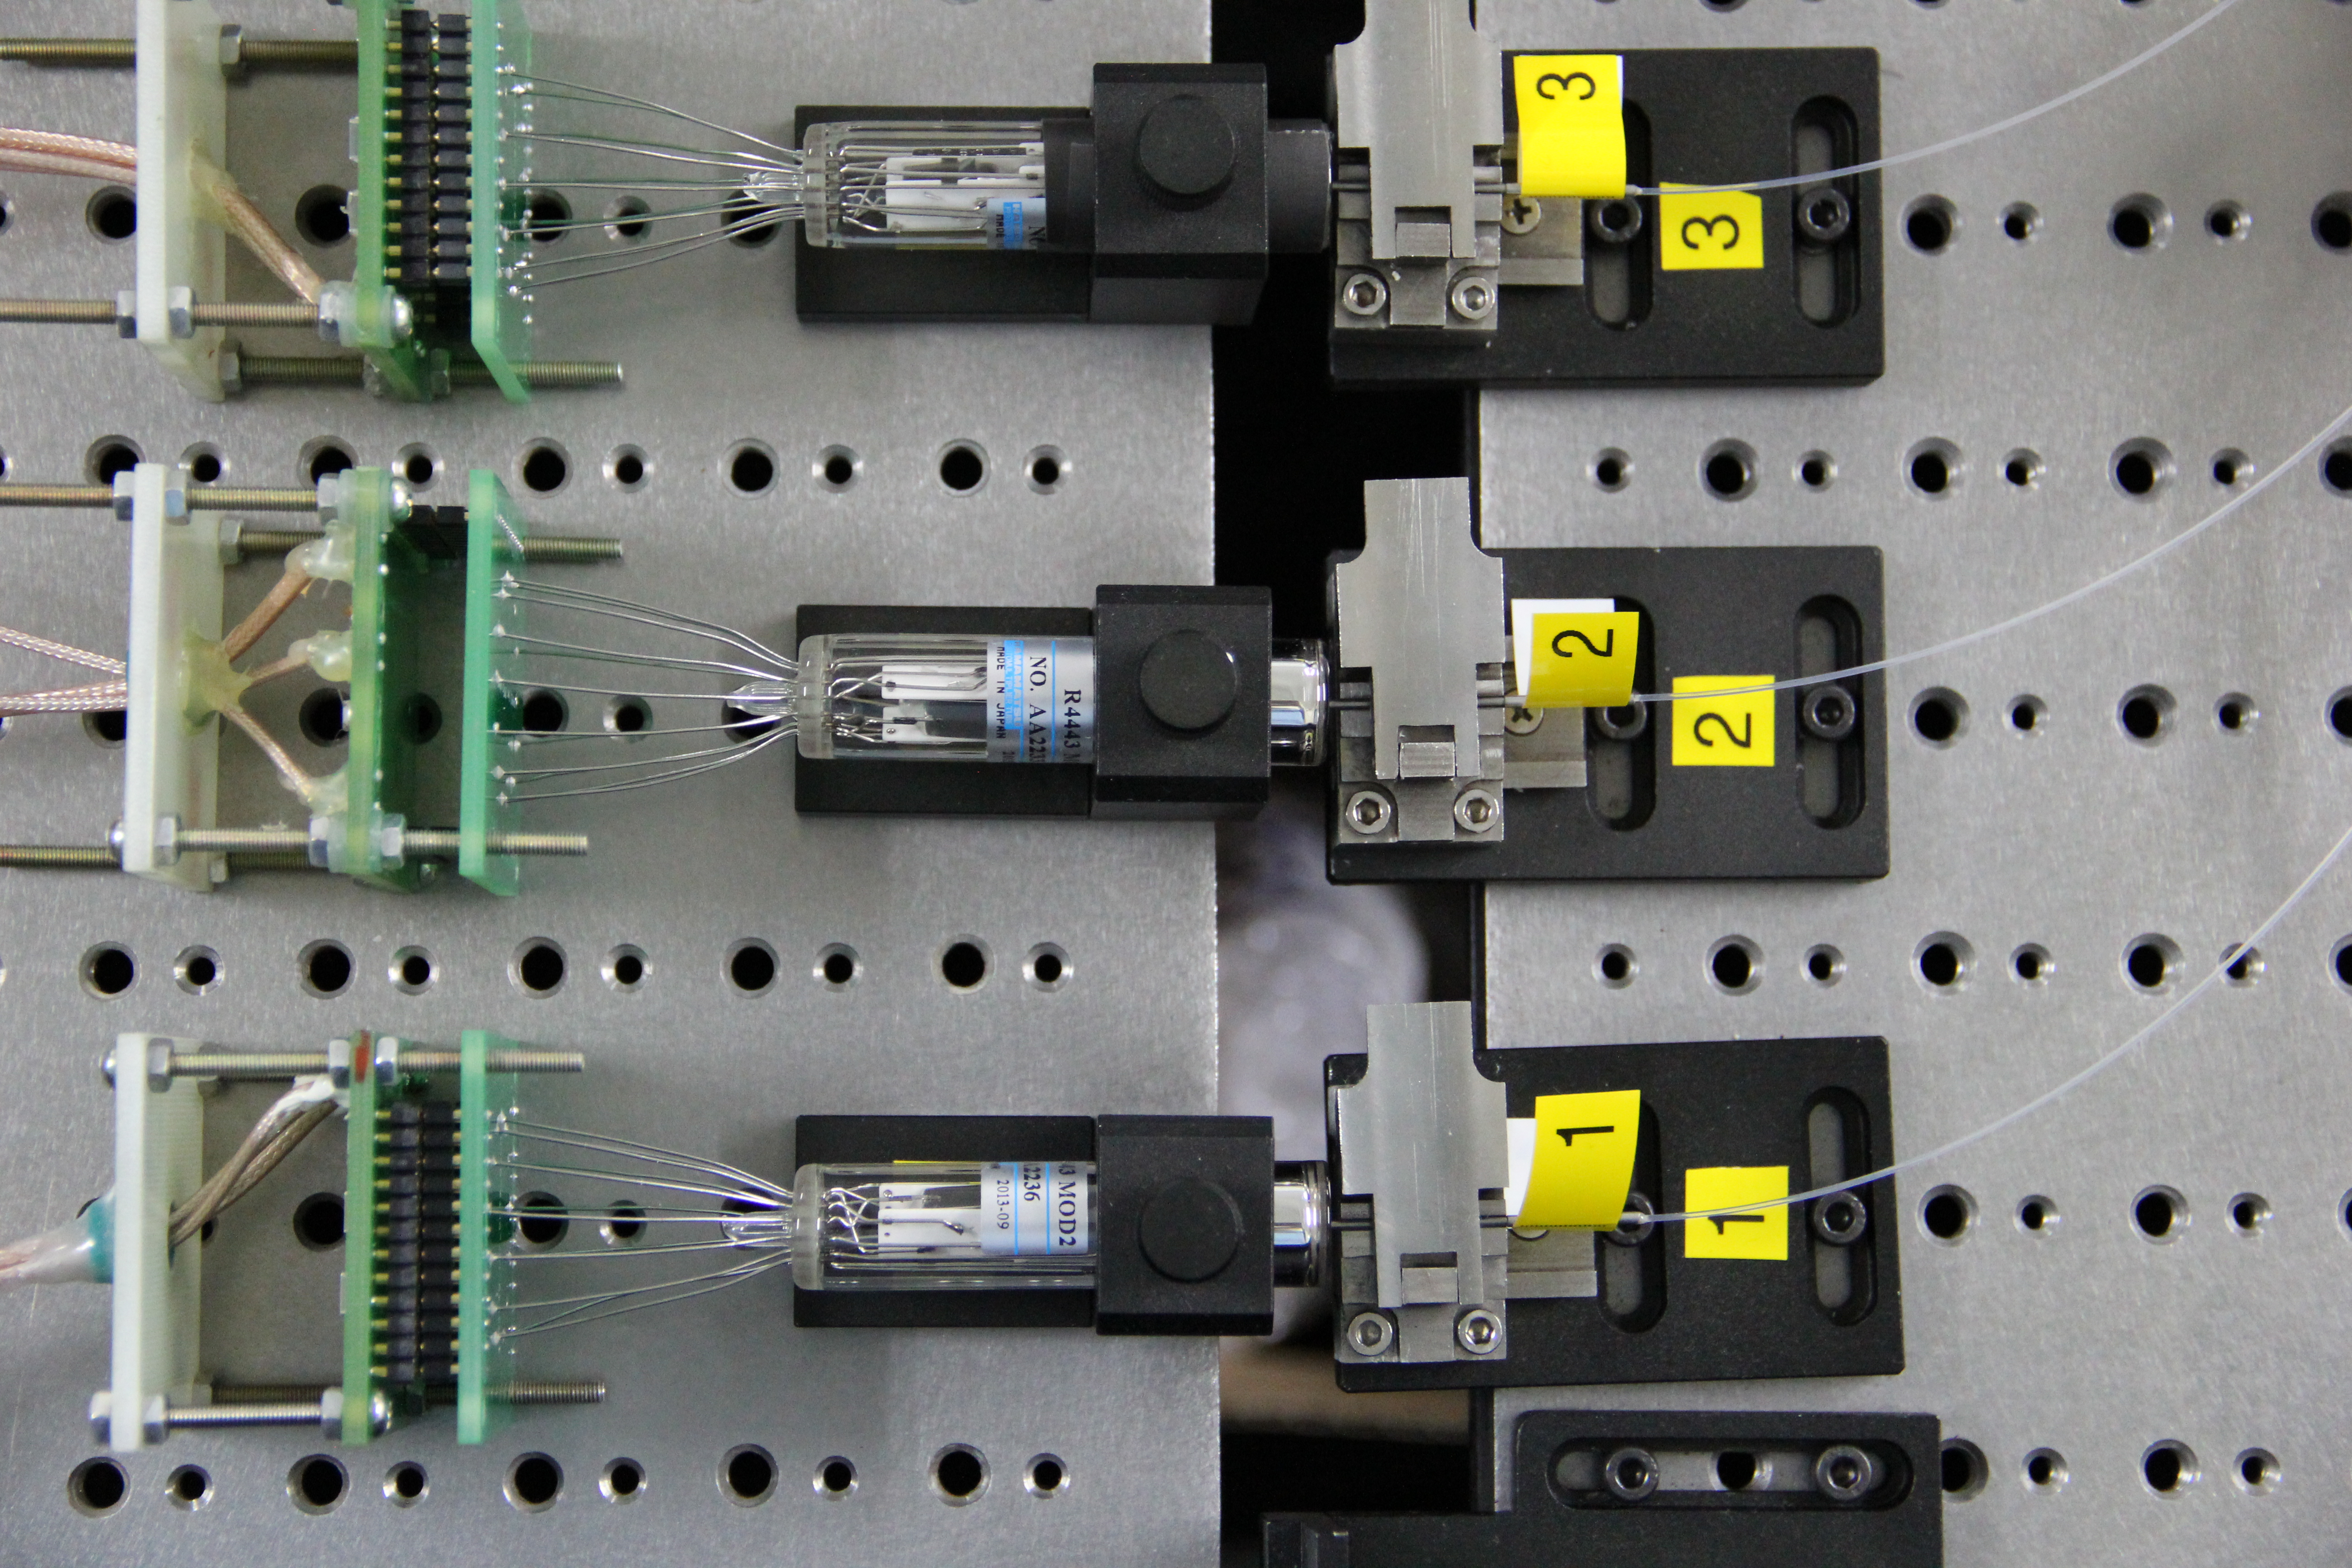
\includegraphics[width=0.6\textwidth]{chap/pmt_test/fig/fixtures.jpg}
	\caption{PMT夹具和光纤夹头}
	\label{fig:pmt_test:fixtures}
\end{figure}

% 光源以及驱动
PMT测试系统使用大功率的蓝光LED(\SI{3}{\watt}, \SIrange{465}{485}{\nano\meter})作为光源。
该LED的发光光谱能够与大部分光阴极材料的光谱响应相吻合,而且曾被成功应用到HIRFL-RIBLL2外靶终端的中子墙光刻度系统中\cite{yuyuhong_led},其功率大小能够满足大量光通路的驱动要求。
为了使LED产生脉冲光,我们采用通用的脉冲发生器AFG3252\cite{afg3252}产生的方波信号来直接驱动LED发光。
虽然AFG3252不是专用的LED驱动器,但它的驱动效果能够满足我们的基本需求,如图\ref{fig:pmt_test:led_pulse}所示。
\begin{figure}[htbp]
	\centering
	\includegraphics[width=0.65\textwidth]{chap/pmt_test/fig/led_pulse.jpg}
	\caption{\SI{30}{\nano\second}脉宽,\SI{5}{\nano\second}上升沿/下降沿的方波脉冲驱动LED发光得到的R4443输出波形}
	\label{fig:pmt_test:led_pulse}
\end{figure}
AFG3252的驱动脉冲参数可以在很大的范围内进行调整,而且精度很高,这是专用的LED驱动器达不到,因此可以满足各种各样的光输出要求,增强了PMT测试平台的通用性。
图\ref{fig:pmt_test:led_response}给出了不同脉宽、不同幅度的方波产生的LED光强变化,可以看到脉冲幅度与LED的输出光强并不成正比,这需要在使用中特别加以注意。
\begin{figure}[htbp]
	\centering
	\includegraphics[width=0.7\textwidth]{chap/pmt_test/fig/led_response.eps}
	\caption{LED输出脉冲的光强度与AFG3253脉冲幅度的非线性关系}
	\label{fig:pmt_test:led_response}
\end{figure}
AFG3252的另外一个优点是:它的所有功能都可以在远程进行控制,而且接口丰富,我们可以选择熟悉的方式对其进行控制。
在PMT批量测试系统中,我们通过网口,并使用SCPI(Standard Commands for Programmable Instruments)命令\cite{afg3000_programmer_manual}对AFG3252进行远程操作。

% 积分球
LED发出的光脉冲通过集束光纤被分配到各支PMT,它与集束光纤之间通过一个\SI{5}{\centi\meter}的积分球耦合。LED、积分球和集束光纤一起构成了PMT测试系统的光分配系统,如图\ref{fig:pmt_test:light_distribution}。
其中LED通过导热硅胶固定在一个与积分球入射端口适配的底座上,而集束光纤通过三维位移台直接对准积分球出射端口的中心(参加见图\ref{fig:pmt_test:lightsource_integration})。
\begin{figure}[htbp]
	\centering
	\subfloat[][1)LED 2)积分球 3)集束光纤]{
		\label{fig:pmt_test:lightsource_components}
		\includegraphics[width=0.49\textwidth]{chap/pmt_test/fig/lightsource_components.jpg}
	}
	\subfloat[][各组件耦合在一起]{
		\label{fig:pmt_test:lightsource_integration}
		\includegraphics[width=0.49\textwidth]{chap/pmt_test/fig/lightsource_integration.jpg}
	}		
	\caption{PMT批量测试平台的光源与光分配系统}
	\label{fig:pmt_test:light_distribution}
\end{figure}
积分球是一个具有高反射性内表面的空心球体,它是一个理想的光积分器件,入射光在其内部经过多次反射后,能够在其出射端口均匀出射。
积分器在此处的应用主要出于两点考虑:1)我们希望各条光通路具有相近的光输出强度;2)方便积分球与集束光纤之间的耦合操作,减弱LED光源的非均匀性对各光路输出强度差异的影响。
我们使用的积分球\cite{integrating_sphere}使用的内壁涂层材料为$BaSO_4$,蓝光反射率达到\SI{98.5}{\percent},因此即便它的半径较小,仍然能够得到较好的均匀性。
在LED固定到积分球入射端口后,我们对积分球出射端面的光强度进行了“十”字扫描,结果显示其光均匀性可以达到$\pm\SI{0.5}{\percent}$,如图\ref{fig:pmt_test:integrationsphere_uniformity}所示。
\begin{figure}[htbp]
	\centering
	\includegraphics[width=0.65\textwidth]{chap/pmt_test/fig/integrationsphere_uniformity.eps}
	\caption{\SI{5}{cm}铝合金积分球输出端口的光均匀性}
	\label{fig:pmt_test:integrationsphere_uniformity}
\end{figure}

% 集束光纤
PMT批量测试系统使用的集束光纤由35根塑料包层的石英光纤\cite{optical_fibre}集结而成(25根用于待测光通道,2根用于监控光通道,剩余8根备份)。每根光纤的长度为\SI{1.5}{\meter},纤芯直径为\SI{400}{\micro\meter},包层厚度\SI{75}{\micro\meter},而数值孔径达到了$0.37$。
较大的芯径和数值孔径使得每条光通路都能从积分球中引出足够的光量,并传输到对应的PMT入射端面。
为了避免机械损伤,光纤的两个端头部位都加装了铝合金套筒进行保护,见图\ref{fig:pmt_test:lightsource_components}。
光源和光分配系统固定完成后,我们对35条光通路的输出光强差异进行了测试。
测试使用了两支R4443,一支管子用于监测LED的光强波动,其数值可以对测试结果进行光强校正;另一支管子用于正式测试,它固定不动而待测光纤使用高精度的光纤位移台调整位置,保证每次测试时待测光纤都能对准测试PMT光阴极的相同位置。
测试中,我们使用了两个不同幅度的LED驱动脉冲设置分别对所有光通路进行了扫描。
两种设置虽然有将近4倍的光强差,但它们得到的光强差异是在$\pm \SI{0.3}{\percent}$的范围内是完全一致的,结果如图\ref{fig:pmt_test:fiber_difference}所示。
\begin{figure}[htbp]
	\centering
	\includegraphics[width=0.7\textwidth]{chap/pmt_test/fig/fiber_difference.eps}
	\caption{集束光纤各通道的光传输差异性}
	\label{fig:pmt_test:fiber_difference}
\end{figure}
测试结果显示,所有光通路的输出光强度差异不大,但并不完全一致,其分布的标准差为\SI{10}{\percent}。
考虑到积分球的光输出分均匀性只有\SI{0.5}{\percent},可以认为各光通路的光输出强度差异主要是光纤自身的传输效率差异导致的。
由于传输效率是光纤的固有特征,其在相当长的一段时间内是比较稳定的,可以认为是个常数。
假设本次测试中,编号为$fiberid$的光纤输出光强度为$L_{fiberid}$,同时在所有光通道中选择一个作为参考通道,其输出光强度为$L_{ref}$。
则编号为$fiberid$的光通道的光输出强度差异系数$\tau_{fiberid}$可以定义为:
\begin{equation}
	\tau_{fiberid} = \frac{L_{fiberid}}{L_{ref}}
	\label{eq:pmt_test:lightoutput_difference}
\end{equation}
根据上面的叙述,$\tau_{fiberid}$可以被认为是一个常数,它主要用于对测试数据进行光强校正,使得不同光通道的测试结果可以直接进行比较(详见第\ref{sec:pmt_test:characterization}节)。

\subsection{模块化设计的测控软件}
\label{sec:pmt_test:software}
% 最好这里做一个归纳性的介绍,具体细节设计放到附录中
PMT批量测试平台的测控软件是系统的重要组成部分,它直接关系到平台的易用性。
由于该测试平台被设计为是一个通用的测试系统,我们需要考虑很多潜在的测试内容,并且底层硬件需要经常更换或更新(见\ref{sec:pmt_test:testbench_functions}的描述)。
因此,PMT批量测试平台的测控软件框架采用模块化的设计思路,并对底层硬件进行了封装和虚拟化,从而方便软件进行维护以及扩展。
测控软件框架基于C++语言编写,并在Windows环境下运行,其内部组件可以被分为以下三个层级:
\begin{enumerate}
	\item 设备的抽象层。分别用一个C++的抽象类代表\ref{sec:pmt_test:testbench_functions}节中介绍的四个功能模块,并将各种模块常用的操作抽象出来作为借口函数。任何一个新加入的设备都可以从这四个抽象类中继承出来,并对提供自己接口函数实现。软件框架里的其余部分可以通过这四个抽象类来完成自己的功能,并不涉及其具体实现,从而将底层硬件与顶层功能隔离开来。
	\item 测试算法与辅助功能库。这一层提供了一些基于上述的设备抽象层实现的一些较为通用的测试用例算法,以及一些管理类和辅助功能类。
	\item 用户交互层。这一层主要处理和用户的交互,其具体实现与上两层无关,可以基于命令行,也可以基于图形界面。
\end{enumerate}
测控软件框架的具体设计细节可以参看附录\ref{appendix:pmttest_software},此处略去。
对于PSD的光电倍增管测试来说,我们基于NI-VISA\cite{ni_visa}函数库实现了对PSD地面检测获取系统的控制,以代替通用的CAMAC数据获取模块。
针对PSD的测试需求,实现了Dy8增益测试、Dy5和Dy8的相对增益测试以及光阴极扫描测试这三个测试算法。
最后,我们基于PDCurses\cite{pdcurses}开发了一个命令行交互的测控程序,集成了设备控制,状态监控以及日志记录等功能。

\section{R4443裸管的性能测试}
\label{sec:pmt_test:characterization}
我们使用PMT批量测试平台对
% 分压器
% 高压分组导致从570支 选194 最后用164
% 获取系统组成,数据分析,数据库存储
% 统计信息 20一个run 共28个run 一个月测试完成
% 测试流程: 预热

\subsection{PSD对光电倍增管的测试需求}
由于PSD没有参加DAMPE的触发系统,PSD不需要对粒子的入射时间进行测量。
因此,R4443的时间性能参数没有实际的参考价值,无需在实验室对其进行专门的测试。
另一方面,PSD通过测量沉积能量来实现其所有功能(见第\ref{sec:description:psd_principle}节),而光电倍增管的增益是直接影响探测器能量响应的重要参数。
因此,我们的测试主要关注R4443与增益相关的性能参数,这包括Dy8的增益以及Dy5和Dy8间的相对增益(简称Dy58比值)这两个方面。
% 能量响应均匀性的要求
PSD要求各探测单元模块的能量响应均匀性好于\SI{25}{\percent}。这意味着,需要

% 高压分组使得需要对大量管子进行测试
高压分组的限制

\subsection{相对增益的测量}
% 测试方法的介绍:
Dy8增益小
单光电子峰为电子倍增器的增益,没有包含光阴极的影响。
% 流程、配置介绍

% 结果介绍

\subsection{Dy8和Dy5之间相对增益的测量}
\subsection{光阴极均匀性的测量}

\subsection{PMT批量测试平台的长期稳定性}

\section{PMT的筛选}

\subsection{筛选方案}
工厂参数。
% 暗电流
PMT的暗电流是指在完全黑暗且没有入射光的条件下,在光电倍增管内部流动的微小电流。
由于暗电流会使得探测器的基线展宽、噪声变大,严重的情况下甚至降低探测器的能量分辨率,因此暗电流越小越好。
光电倍增管的光阴极材料是引起暗电流的主要因素。
PSD采用的R4443型号(即MOD2)使用低噪声的碱金属材料作为光阴极,从而极大地抑制了暗电流的大小。
根据Hamamatsu提供的出厂测试信息,我们发现所有管子的暗电流都小于PSD的要求。
% 增益
R4443的Dy8通道用于覆盖PSD动态范围的低端部分,主要用于$e/\gamma$;R4443的Dy5通道用于覆盖PSD动态范围的高端部分,主要用于相对论重离子的电荷测量。
我们希望Dy8的增益尽量高,使其测得的MIP信号尽量与基线噪声相分离,从而降低$e/\gamma$误判率。
另一方面,PSD对整体的动态范围有严格的区间要求($\SI{0.1}{MIPs}\sim\SI{1400}{MIPs}$),过高的Dy8增益会压低Dy5的增益(即提高了Dy58比值),从而降低Dy5对重离子电荷的分辨能力。
因此
\subsection{参考单元模块的MIPs响应}
\subsection{与塑闪单元条的匹配}
	% 各章节。
	\chapter{塑闪阵列探测器的建造与质量控制}

\section{空间环境对探测器建造的特殊要求}

\section{PMT组件的装配}

\section{探测器整体装配}

\section{环境实验}
	%
	\chapter{PSD的宇宙线地面标定}
\label{ch:cosmic_ray}
PSD整体装配完成后,我们在实验室对它的各项性能指标进行了测试。
特别地,我们利用宇宙线对PSD探测单元模块进行了细致的标定测试,得到了一系列的刻度参数结果。
这些结果是PSD得到的第一批刻度参数数据集,它们是PSD进行初步能量重建的基础。

我们专门研制并搭建了一套宇宙线地面标定系统对PSD整体进行标定测试。
本章将简单介绍该系统的基本组成以及它在PSD宇宙线标定中的应用,同时给出了PSD地面宇宙线标定的主要结果。

\section{宇宙线地面标定系统}
\label{sec:cosmic_ray:cm_system}
\subsection{简介}
\label{sec:cosmic_ray:introduction}
% 结构与组成,总装图
% 基本原理
宇宙线地面标定系统是专门为了PSD的地面标定而设计和建造的,主要提供了两个功能:1)模拟轨道真空环境;2)确定入射宇宙线径迹。
该系统的硬件组成如图\ref{fig:cosmic_ray:cm_system}所示,其主体为一个大型真空靶室,靶室大小正好可以容纳整个PSD探测器。
真空靶室的腔体上部和下部分别放置了一个多丝漂移室探测器(Multi-Wire Drift Chamber,简称MWDC)和一个塑料闪烁体触发板探测器。
上下两块大面积触发板用于标定入射宇宙线事例,而上下两个MWDC则用于测量入射宇宙线径迹。
根据得到宇宙线入射径迹,可以推出其在PSD上的击中位置;而MWDC和触发板的面积都能够覆盖PSD的有效面积,因此我们能够得到PSD所有位置处的MIP响应,从而实现PSD的精细标定。
\begin{figure}[htbp]
	\centering
	\includegraphics[width=0.65\textwidth]{chap/cosmic_ray/fig/cm_system.jpg}
	\caption{宇宙线地面标定系统的硬件组成}
	\label{fig:cosmic_ray:cm_system}
\end{figure}

按照功能分类,宇宙线地面标定系统可以被分为真空系统、径迹探测系统、触发系统以及数据获取系统。
下面,依次对各个分系统进行详细介绍。

\subsection{真空系统}
\label{sec:cosmic_ray:vacuum_system}
% 靶室大小,结构包括滑台,外观图
% 高压法兰,信号法兰图
% 真空泵,参数
真空系统主要由靶室、真空泵以及真空检测设备组成。
靶室腔体大小为$TODO$,可以容纳整个PSD探测器;靶室外部支架上设计有托盘,用于固定MWDC和塑闪触发板。
靶室内部还铺设了两根导轨,操作时,我们先将PSD安放在一个铝合金滑台上并准确定位,然后将滑台沿着导轨推入到靶室腔体中,最后将滑台用卡扣卡住以防其滑动。这样不仅方便了PSD的放置操作,而且能够准确定位PSD在靶室内部的位置,为后面的数据分析提供依据。
为了给靶室内部的PSD提供高压并将其信号引出,我们专门加工了PSD专用的高压转接法兰和信号转接法兰,如图TODO所示。

真空系统中的真空泵设备由机械泵和分子泵两级组成,以保证靶室内部可以达到较高的真空度。
相应的,真空检测设备也分为TODO。
由于靶室体积较大,我们配备了两套相同的真空泵设备以加快抽真空的速度。
实际使用中发现:当靶室内部放置了PSD探测器和相应的连接线缆后,TODO小时内可以将靶室内部真空抽取最低值多少。

\subsection{径迹探测系统}
\label{sec:cosmic_ray:tracking_system}
% MWDC工作原理
MWDC是气体探测器的一种,由于制造成本低廉、操作简单以及位置分辨较高,它是粒子物理实验中最常用的位置灵敏探测器之一。
MWDC一般由多个漂移单元组成,每个漂移单元都是MWDC进行位置测量的最小单位。
一个漂移单元由位于中心的一根阳极丝和周围的若干根阴极丝组成;工作时,阳极丝加正高压(或接地),而阴极丝接地(或加负高压);阴极丝也被称为场丝,因为它们的排布方式决定了漂移单眼内部的电场分布。
入射粒子穿过漂移单元时,在其中发生的物理过程可以叙述如下:
\begin{enumerate}
	\item 入射粒子使得单元内的气体分子电离,从而产生自由的电子离子对。
	\item 在电场作用下,电离出来的电子被加速并缓慢向阳极丝漂移,而离子则向阴极丝移动。
	\item 由于阳极丝附近电场强度非常大,自由电子漂移到这个区域以后迅速被加速到足够高的能量并能够引发新的电离。这个过程不断地反复地进行,从而产生大量电离电子,这个现象被称为雪崩效应。
	\item 雪崩效应产生的自由电子继续向阳极丝移动,由于距离阳极丝非常近,它们立即被阳极丝收集。
	\item 与此同时,原初电离以及次级电离产生的正离子继续向阴极丝移动,由于离子的质量大,它们的漂移速度很慢,而且也不会在阴极丝附近产生雪崩效应。
\end{enumerate}
上述各个步骤中,只有大量雪崩电子向阳极丝移动并被迅速吸收这个过程能够使得阳极丝上的电荷分布发生变化并感应出幅度可探测的电流脉冲信号。
MWDC探测到的也就是这个阳极丝上的感应电流信号,该信号产生时刻与入射粒子穿过漂移单元的时刻的时间差就是原初电离电子的漂移时间。
由于漂移距离与漂移时间直接关联,通过测量漂移时间可以反推出原初电离位置相对于阳极丝的位置,这就是MWDC进行位置测量的基本原理。

% 基本结构:面积,丝参数,精度。
% MWDC结构示意图(丝距离,丝面排布)
% MWDC实物图
径迹探测系统由两个完全一样的平面MWDC探测器组成。
每个MWDC探测器由X,Y,U三个方向的漂移单元平面阵列组成,其有效探测面积为$840mm \times 840mm$。
X面与Y面成\SI{90}{\degree}排布,它们内部都有80个漂移单元;U面与X面成\SI{30}{\degree}排布,它的内部有106个漂移单元,如图TODO所示。
漂移单元平面阵列是由两个阴极面和一个阳极面构成的,面间距为\SI{5}{mm}。
其中,阴极面由直径为\SI{100}{\micro\meter}的铍铜丝紧密排列组成,而阳极面由直径为\SI{100}{\micro\meter}的铍铜丝和直径为\SI{20}{\micro\meter}的镀金钨丝间隔排列组成,如图TODO所示。
\begin{figure}[htb]
\centering
\subfloat[][焊接第一块Base板]{
	\label{fig:construction:soldering_a}
	
\includegraphics[width=0.48\textwidth]{chap/cosmic_ray/fig/mwdc_planes.png}
}
\subfloat[][焊接第二块Base板]{
	\label{fig:construction:soldering_b}
	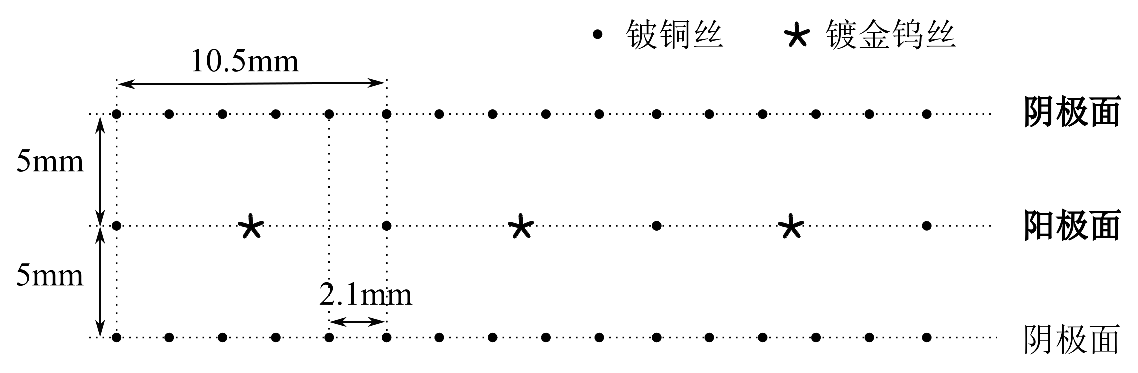
\includegraphics[width=0.48\textwidth]{chap/cosmic_ray/fig/mwdc_wire_pattern.eps}
}
\caption{R4443的Base电路板焊接流程}
\label{fig:construction:soldering}
\end{figure}
工作时,所有的铍铜丝加负高压,它们是漂移单元的阴极丝;所有的镀金钨丝接地,它们是漂移单元的阳极丝。
因此,根据图\ref{}给出的间距,可以得到MWDC的漂移单元是一个截面为$10mm\times 10.5mm$的长方体。
MWDC探测器的工作气体为$\SI{20}{\percent}CO_2 + \SI{80}{\percent}Ar$,整个漂移腔体用Kapton膜密封,图TODO给出了一个MWDC探测器的实物图。
\begin{figure}[htbp]
	\centering
	\includegraphics[width=0.65\textwidth]{chap/cosmic_ray/fig/mwdc.jpg}
	\caption{MWDC实物图}
	\label{fig:cosmic_ray:mwdc}
\end{figure}
% MWDC的信号处理系统
MWDC的输出信号幅度较小,为了提高信噪比,我们使用一块基于SFE16芯片的前端电子学板对原始信号进行预处理,然后才将其输出到数据获取系统中进行时间测量(见\ref{sec:cosmic_ray:daq_system}节)。
SFE16是一款专门用于气体漂移室前端信号处理的低噪声ASIC芯片。
它将16个测量通道集成在一块芯片上,每个通道都具有信号放大和甄别的功能,因此输出信号可以直接用于时间测量,并适合长距离传输。
关于SFE16的详细信息可以参考文献\cite{sfe16}。

\subsection{触发系统}
\label{sec:cosmic_ray:triggering_system}
% 触发板结构,面积,厚度,四角读出,实物图?
触发系统由两块完全一样的塑料闪烁体触发板探测器组成。
触发板探测器使用\SI{30}{mm}厚的塑料闪烁体EJ-200\cite{ej-200}作为探测介质,探测器形状为正方形,有效面积为$825mm \times 825mm$。
塑闪板表面抛光,并在内层包裹Tyvek纸以提高反射效率,而在外层包裹黑胶带以屏蔽外界的光干扰。
最后,塑闪板的四个角各耦合了一支光电倍增管,用于闪烁光信号读出,如图TODO所示。
使用的光电倍增管型号为Hamamatsu公司的R7724\cite{r7724}。

% 触发板的信号处理系统
触发系统具有两个功能:1)标识入射宇宙线,为数据获取系统提供触发信号;2)用于宇宙线击中时刻的测量,为MWDC漂移时间的计算提供时间零点。
上下两块触发板探测器共有8路信号输出,相应地,它们经过甄别后可以得到8路时间信号。
每一路时间信号都扇出两路,一路信号参加8路时间信号的逻辑与运算;另一路信号用于时间测量。
上述两个功能都在同一块信号处理板中实现,详细内容参看\ref{sec:cosmic_ray:daq_system}节。
我们认为真实的宇宙线事例应该使得上下两块触发板都点火,因此8路信号相与得到的输出信号将作为触发信号输入到数据获取系统中以记录该事件。
而8个角上得到的时间测量值将被用于漂移时间零点的计算。

% 响应均匀性,击中位置图或者唐述文文章中的图
由于触发板的面积较大,宇宙线击中板上不同位置处产生的闪烁光传输到塑闪板上同一支PMT的时间是有差异的,我们把这个现象称为时间测量不均匀性,如图\ref{fig:cosmic_ray:tof_timeVSposition}所示。
\begin{figure}[htbp]
	\centering
	\includegraphics[width=0.65\textwidth]{chap/cosmic_ray/fig/tof_timeVSposition.png}
	\caption{触发板的时间测量不均匀性,引自\cite{tang_large_2015}。其中,纵轴是某个角得到的击中时刻,而横轴是击中位置距离这个角的直线距离。拟合直线斜率的倒数就是闪烁光在塑闪板中的有效传播速度。}
	\label{fig:cosmic_ray:tof_timeVSposition}
\end{figure}
这意味着,我们不能简单地选择一支PMT的时间信号作为时间零点,因为这会带来较大的时间晃动,影响漂移时间的测量精度。
为了消除时间测量不均匀性,必须综合板上四个角的时间测量信息,以使得时间零点与击中位置无关。
实际中,我们使用下列形式\cite{annand_large_1987}得到时间零点$T_{eff}$:
\begin{equation}
	T_{eff} = \frac{1}{4}\sum^4_{i=1}T_i - \frac{v_{eff}}{8d}[(T_3-T_1)^2+(T_4-T_2)^2]
	\label{eq:cosmic_ray:tof_time}
\end{equation}
其中,$v_{eff}$是闪烁光在塑闪板中有效传输速度,$d$是塑闪板的对角线长度,$T_1\sim T_4$是塑闪板四个角的时间测量值,并且$T_1和T_3$是对角,而$T_2和T_4$也是对角。
测试发现,使用公式\ref{eq:cosmic_ray:tof_time}得到的塑闪板时间分辨率可以达到\SI{350}{\pico\second}\cite{tang_large_2015}。

\subsection{数据获取系统}
\label{sec:cosmic_ray:daq_system}
% PXI机箱图,触发板,MWDC板,TOF板
数据获取系统基于PXI总线设计,主要由触发板,时钟板,TOF测量板以及MWDC测量板组成。
这些板卡都安装在一个6U高,具有15个槽位的PXI机箱中\cite{TODO},而获取和控制软件安装在机箱第一个槽位的单片机上。
下面,对这四种板卡的功能进行简单的介绍。

TOF测量板和MWDC测量板是数获取系统进行时间测量的核心模块,其中TOF板用于触发板探测器的时间测量,而MWDC板用于MWDC探测器的时间测量。
两块测量板都是基于HPTDC芯片设计的,能够在高计数率条件下对时间进行精确测量。
HPTDC是欧洲核子中心(CERN)开发的一款高性能时间测量ASIC芯片\cite{TODO}。
与以往核物理实验中常见的起停式时间测量方法不同,HPTDC直接测量输入时间信号的到达时刻,而不是测量输入时间信号与触发信号的时间差。
HPTDC也需要触发信号,但它并不将触发信号作为时间测量的零点,而是使用触发信号来寻找真实的时间测量值,具体流程如下:
\begin{enumerate}
	\item 首先,所有输入到HPTDC的时间信号,不管是真实物理事件产生的还是本底噪声产生的,它们的到达时刻都会被测量并暂时保存到芯片的信号缓存中。
	\item 之后,触发信号输入到HPTDC中,其到达时刻也被测量并暂时保存到触发信号缓存中。
	\item 由于触发信号代表真实的物理事件,它的产生时刻与真实待测的时间信号之间必定满足一定的时间关系,其中包括各种电子学和线缆的延迟时间。这个关系可以用一个时间窗口来表示,并可以在实验前通过模拟和测试估算出来。用户在实验开始前,需要将这个关系配置保存到在HPTDC的配置寄存器中。
	\item 实验中,HPTDC就是根据这个配置好的时间窗口,从信号缓存中已有的时间测量值中找到每个触信号对应的真实时间测量值,并将其输出到读取FIFO中,供获取软件使用。
\end{enumerate}
由于HPTDC会将所有满足时间窗口的测量值都提取出来,因此需要仔细调节时间窗口配置以达到每个触发信号只能找到一个测量值的最佳状态。
这给实验准备提出了更高的要求,但这种测量方法具有死时间小、配置灵活等优点,非常适合复杂探测系统在高计数率条件下的使用。
HPTDC具有32个测量通道,每个通道的时间测量精度为\SI{100}{\pico\second};HPTDC也可以工作在精度为\SI{25}{\pico\second}甚高精度模式下,此时每4个测量通道合并成1个测量通道,即此时HPTDC只有8个测量通道。
TOF板共有16个测量通道,其内部共使用了3片HPTDC,其中两片用于时间测量,工作在甚高精度模式下,一片用于TOT幅度测量(Time-Over-Threshold),工作在正常模式下。
MWDC板共有128个测量通道,其内部使用了4片HPTDC,全部工作在正常模式下。
对于
% \section{多丝漂移室的宇宙线刻度}
% \subsection{漂移时间零点的确定}
% \subsection{从漂移时间谱提取s-t关系:Integration Method}
% \subsection{迭代修正s-t关系}
% \subsection{多丝漂移室的性能参数}

\section{PSD的宇宙线标定}
% 15天,23个/s,一共事例数? 27%左右的单根丝点火事例
% 与PSD系统的集成,触发Veto板。
% 触发板预支设置,击中分布图
\label{sec:cosmic_ray:cm_test}
\begin{figure}[htbp]
	\centering
	\includegraphics[width=0.65\textwidth]{chap/cosmic_ray/fig/cm_test.jpg}
	\caption{PSD的宇宙线标定测试}
	\label{fig:cosmic_ray:cm_test}
\end{figure}

\section{标定结果}
\label{sec:cosmic_ray:results}
\subsection{基线噪声}
加高压与未加高压的结果对比。
基线中心值。
电子学刻度?

\subsection{MIP响应}
中心MIP拟合示例图
中心值一致性
能量分辨率分布

\subsection{光衰减效应}

\subsection{Dy58比值}
拟合示例
分布图,与LED测试值对比
动态范围计算与分布

\subsection{探测效率}
探测效率判据
事例筛选
结果分布

\subsection{位置分辨}
位置重建原理
结果

\section{PSD的物理量重建研究}
\subsection{能量重建}
\subsection{位置重建}
	% 各章节。
	\chapter{PSD在CERN-SPS的重离子束流标定}

\section{实验简介}
\subsection{实验条件}
\subsection{辅助探测器与实验布局}
\subsection{次级束的产生}
\subsection{$\Delta E$-$\Delta E$重离子鉴别方法}
\subsection{数据分析}

\section{PSD的重离子响应}
\subsection{Dynode8/Dynode5比值的线性}
\subsection{重离子的光输出}
\subsection{光衰减效应}
\subsection{不同单元模块的响应均匀性}

\section{PSD的电荷分辨能力}
\subsection{单元模块的电荷分辨率}
\subsection{PSD整体的刻度与能量重建}
\subsection{PSD的电荷自分辨}

\section{结论}
	% 结论
	% vim:ts=4:sw=4
% Copyright (c) 2014 Casper Ti. Vector
% Public domain.

\chapter{总结与展望}
\label{ch:conclusion}

\section{总结}

DAMPE卫星自2015年12月17日发射并进入轨道后,已经完成了三个月的在轨测试阶段,并正式进入到巡天观测模式。
在轨测试期间,PSD探测器整体工作正常,各项性能指标符合设计要求并非常稳定,从而验证了PSD的设计合理性,并说明PSD建造过程的质量控制过关。

本论文完整展现了PSD从整体设计、组件原理验证、探测器建造以及宇宙线标定的整个研制过程。
其中,论文的主要工作集中在细致研究了影响PSD探测性能的几个关键技术,完成了PSD的建造,并对PSD整体进行了地面宇宙线标定。
另外,论文工作过程中还完成了两套大型的探测器辅助测试平台的设计和研制,这些测试平台为PSD的研制成功提供了坚实的基础。
下面,对本论文取得的主要成果进行一个小结:
\begin{enumerate}
	\item PSD关键技术的细致研究:
	\begin{itemize}
		\item PSD需要覆盖接近4个量级的动态范围区间,这是PSD探测器主体功能模块的主要设计难点。本论文完成了基于Dy5和Dy8双打拿极信号引出的大动态范围读出方案的设计与实验验证,结果显示该设计方案能够满足PSD的动态范围要,并最终应用到PSD的正样飞行件上。
		\item PMT的工作状态直接关系到PSD探测单元模块的性能,大规模的探测器系统中往往需要对大量的PMT进行测试并进行筛选,对于PSD来说此项筛选流程更加严格。本论文对570支候选R4443裸管进行了测试,使用相对增益测量方法得到了它们的增益特性曲线,同时也得到了绝对的Dy58比值增益特性曲线。根据PSD的特殊要求,本论文确定了严格的筛选条件,并根据PMT的测试结果进一步从570支PMT中挑选出164支安装到PSD上。
	\end{itemize}
	\item PSD的建造:探测器的建造相对来讲是一个较为琐碎的过程,然后PSD的建造过程中涉及了大量的工艺和质量测试程序,使得它可以单独成为一个系统,并直接决定PSD最终的探测器性能。本论文的工作完整参与了PSD的整个建造流程。
	\item PSD的宇宙线测试:本论文对装配完成的PSD进行了长度15天的宇宙线测试,并从中提取除了PSD的性能参数,发现PSD的实际性能达到并好于设计指标;另外,本文还从宇宙线标定数据中提取出了PSD的第一批刻度数据,这些数据对于研究PSD的能量重建和模拟具有重要价值。
	\item 大型辅助测试平台的研制:
	\begin{itemize}
		\item PMT批量测试平台是本论文为PSD的R4443测试专门设计和建造的,它最多能够同时测量25支PMT,并具有光阴极扫描功能。考虑到在日常的探测器研制过程经常会有PMT测试工作,本论文对该平台采用模块化设计,其硬件组件和软件组件都很容易更换或更新以适应新的应用需求。
		\item 地面宇宙线标定测试平台是本论文为PSD的宇宙线标定专门设计和建造的,并用它完成了PSD的初次宇宙线刻度。同样的,该测试平台也适合在其它探测器的研制过程中使用。
	\end{itemize}
\end{enumerate}

\section{展望}
PSD的研制工作随着DAMPE的发射成功以及在轨测试的顺利完成而圆满结束。
现在,DAMPE已经进入正式的物理观测模式,每天都是大量的数据下传,同时也意味着对PSD的研究中心将转向物理量的精细重建上,主要有:
\begin{enumerate}
	\item 完成PSD每个探测单元模块的精细能量重建,包括光衰减效应的修正,两端的能量信息提取及综合等。
	\item 完成PSD探测器整体的能量重建,包括击中交叠单元模块的事件处理,量能器反照粒子的干扰去除等。
	\item 完成PSD的Geant4模拟中的数字化工作。
	\item 实现PSD的$e/\gamma$分辨算法,这需要利用STK的重建径迹以及BGO的簇射形状重建。
	\item 完成PSD的在轨标定工作,包括MIPs响应,Dy58比值,电子学刻度,基线以及这些量随环境参数的变化等。
\end{enumerate}

	% special chapter没有章节编号,在目录中显示
% 	\subimport*{chap/special}{}
	% 正文中的附录部分。
	\appendix
	% 排版参考文献列表。
	\printbibliography[
		% 使“参考文献”出现在目录中;如果同时要使参考文献列表参与章节编号,
		% 可将“bibintoc”改为“bibnumbered”。
		heading = bibintoc,
		% 单独设定排序方案。此设定会局部覆盖之前的全局设置。
		% 注:只有同时使用 2.x 或之后版本的 biblatex 和相应兼容版本的 biber,
		% 才能对每个 \printbibliography 命令采用不同的排序方案,
		% 否则只能在载入 biblatex 宏包时就(全局)指定排序方案。
		% 在这样的情况下,请去掉所有的 sorting 选项,否则可能出错。
		% 此外,biblatex 3.0 中 \printbibliography 的 sorting 选项失效,
		% 详见 biblatex-caspervector 的文档。
		sorting = ecnty
	]
	% 各附录。
	% vim:ts=4:sw=4
% Copyright (c) 2014 Casper Ti. Vector
% Public domain.

\chapter{PMT批量测试平台控制软件的设计}



	%\chapter{MWDC的刻度}
	
	
	% 以下为正文之后的部分,默认不进行章节编号。
	\backmatter
	
\end{document}

